\chapter{Tests and results} \label{tests}
\section{Introduction}
This chapter focuses on tests that were run to provide feedback on performance of implemented system and the accuracy of used algorithms with different parameters. 

\section{Performance of algorithms in parallel processing} \label{parallel-performance}
First set of tests includes performance measurements on 32-core processor. Each part of the implementation was run in multiple configurations to observe effectiveness of parallelization.

Tests were using corpuses that contained 10, 100, 1000 and 10000 documents and were run on range of processor cores from 1 to 20.

Each test case was run 10 times and the average of measured times was used for final results. In order to ensure consistency between tests, assumptions were made:
\begin{itemize}
	\item k=10 for kNN
	\item k=10 for k-means
\end{itemize}

\begin{figure}[ht]
\begin{center}
 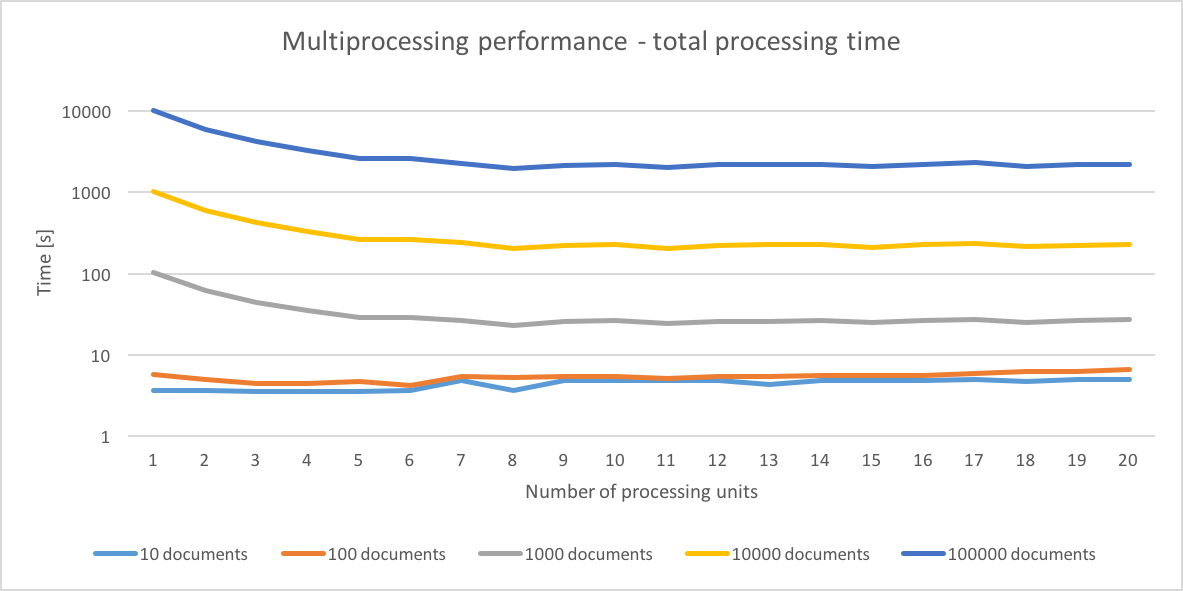
\includegraphics[width=0.9\linewidth]{images/tests/mp-total-sum.png}
 \caption{Overall system multiprocess performance }
 \label{mp-total-sum}
 \end{center}
 \end{figure}
 
\begin{figure}
\begin{center}
 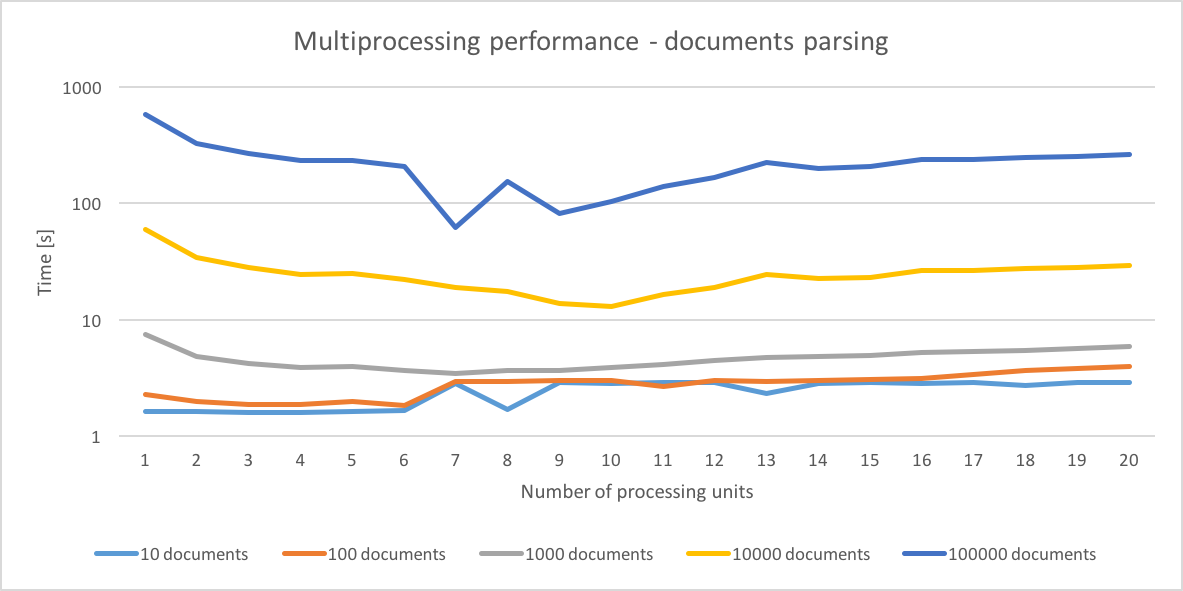
\includegraphics[width=0.9\linewidth]{images/tests/mp-doc-parsing.png}
 \caption{Document parser module multiprocess performance}
 \label{mp-doc-parsing}
 \end{center}
 \end{figure}
 
 \begin{figure}
\begin{center}
 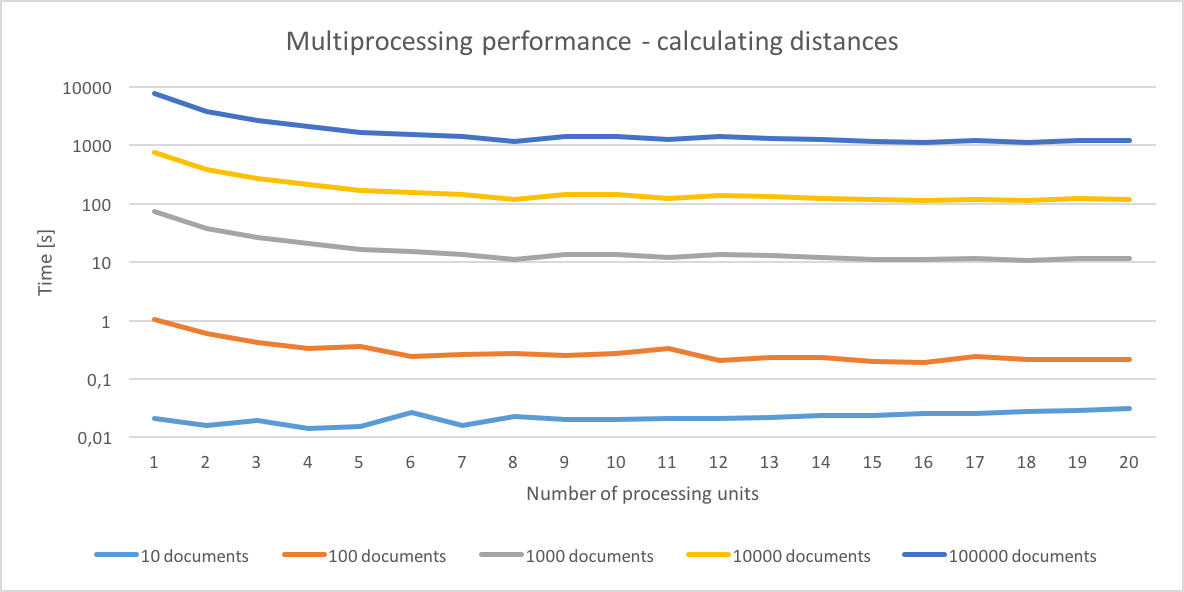
\includegraphics[width=0.9\linewidth]{images/tests/mp-distances.png}
 \caption{Distance calculation module multiprocess performance}
 \label{mp-distances}
 \end{center}
 \end{figure}
 
  \begin{figure}
\begin{center}
 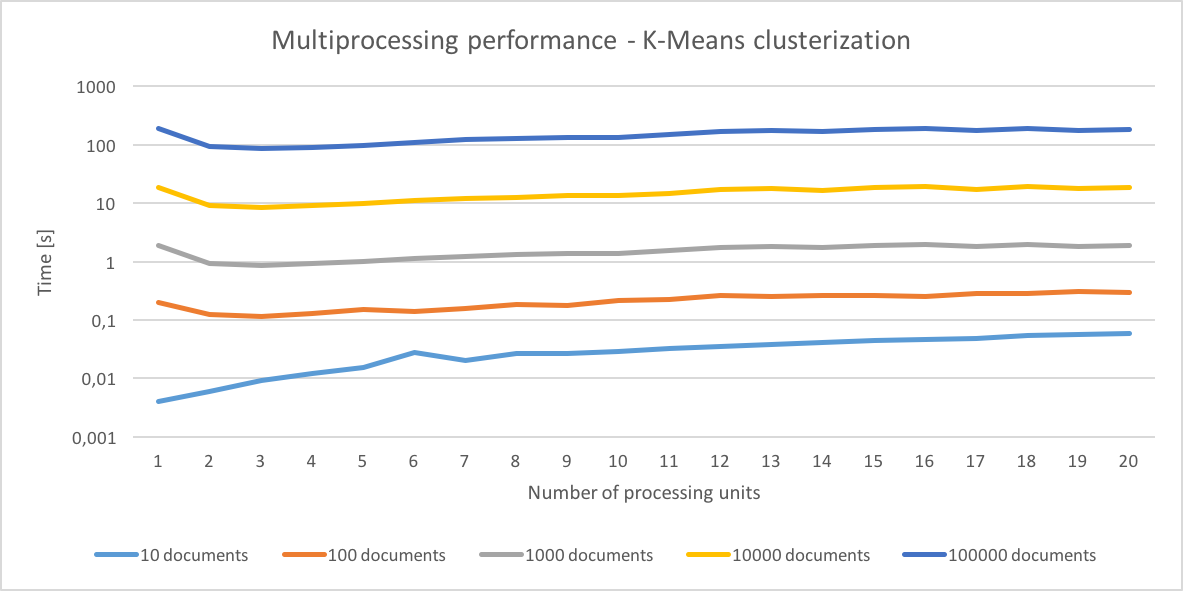
\includegraphics[width=0.9\linewidth]{images/tests/mp-kmeans.png}
 \caption{K-means clustering module multiprocess performance}
 \label{mp-kmeans}
 \end{center}
 \end{figure}
 
  \begin{figure}
\begin{center}
 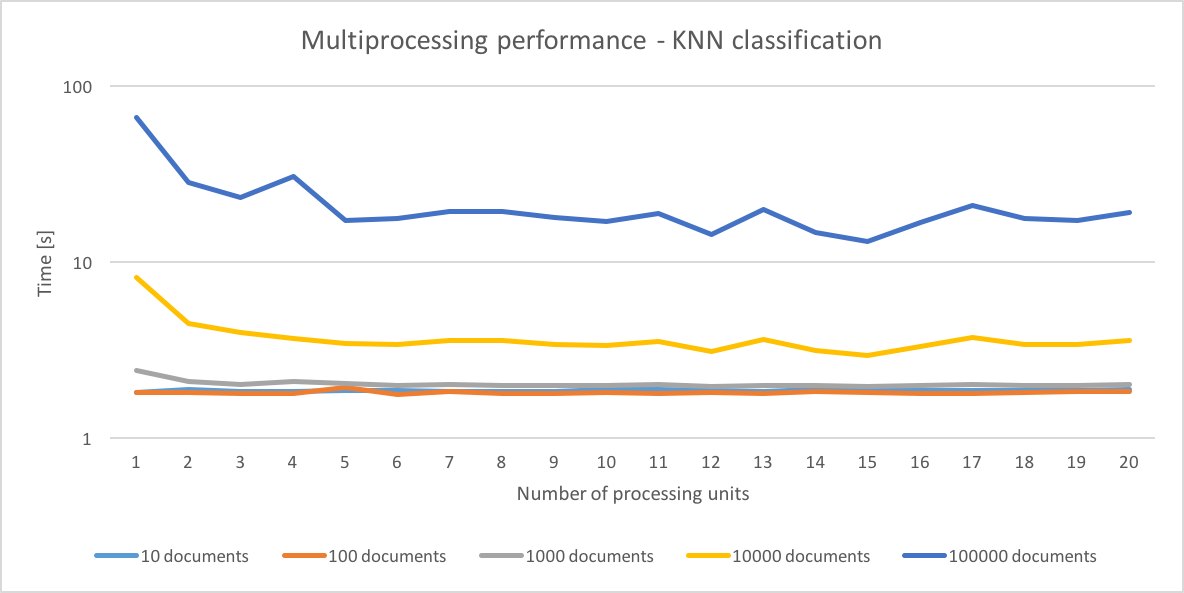
\includegraphics[width=0.9\linewidth]{images/tests/mp-knn.png}
 \caption{ kNN classification module multiprocess performance}
 \label{mp-knn}
 \end{center}
 \end{figure}

\begin{figure}
\begin{center}
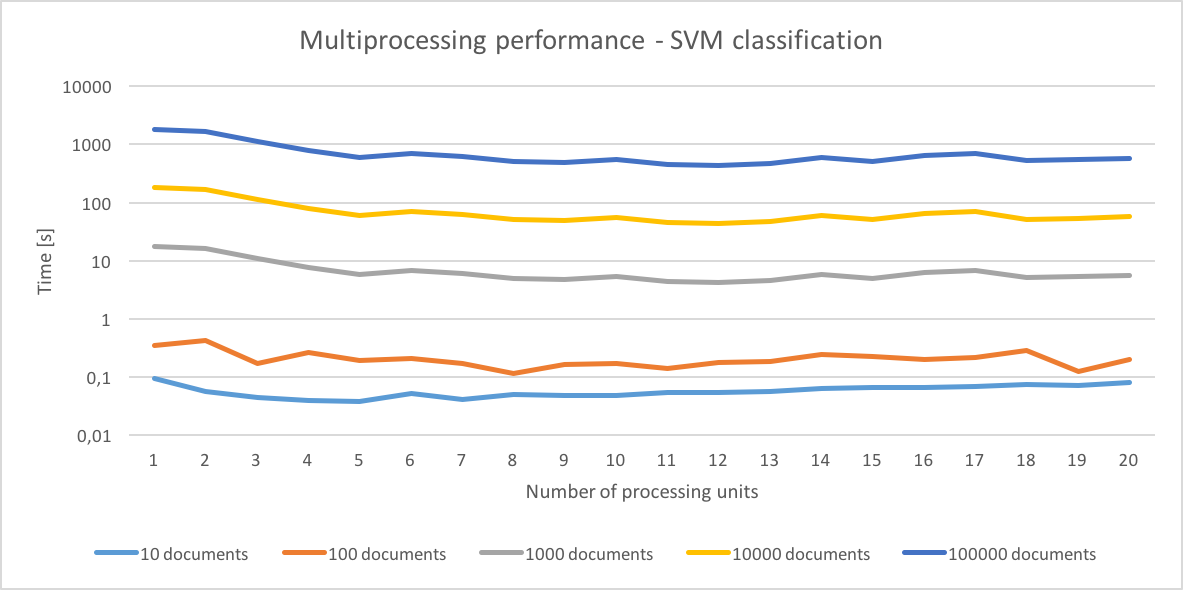
\includegraphics[width=0.9\linewidth]{images/tests/mp-svm.png}
\caption{SVM classification module multiprocess performance }
\label{mp-svm}
\end{center}
\end{figure}

Across all perforrmance tests presented on charts above (\ref{mp-total-sum}, \ref{mp-doc-parsing}, \ref{mp-distances} \ref{mp-kmeans}, \ref{mp-knn}, \ref{mp-svm}, \ref{param-kmeans}, \ref{param-knn} and \ref{param-svm}) it can be noticed that the best performance gain is when around 6 worker processes are working upon completing tasks. Using more workers than that results in no further gains and constant processing time, or even makes processing longer. Main limiting factor that has to be taken into account is communication overhead - a lot of data has to be transfered between processes and at some point master process is not efficent enough to schedule tasks and receive results from workers.

\section{Classification accuracy} \label{classification-accuracy}

For testing classification accuracy true-positive ratio (TP, \ref{TPR}) and false-negative ratio (FN, \ref{FNR}) values were calculated for each of presented classification algorithms. Defining whether document has been classified properly by kNN and SVM algorithms was conducted by external expert with arbitrary knowledge.

In order to ensure consistency between tests, some assumptions were made:

\begin{itemize}
	\item k=20 for kNN
	\item k=300 for k-means
	\item 1000 documents in corpus
\end{itemize}

% \usepackage{booktabs}
% \usepackage{multirow}
\begin{table}[H]
	\centering
	\caption{kNN and SVM effectiveness with different K value in k-means}
	\label{tests:param:kmeans}
	\begin{tabular}{@{}lllll@{}}
		\toprule
		\multicolumn{2}{l}{K value in k-means}     & 75   & 150  & 300  \\ \midrule
		\multirow{2}{*}{kNN} & TP & 0,79 & 0,81 & 0,81 \\
		& FN & 0,21 & 0,19 & 0,19 \\
		\multirow{2}{*}{SVM} & TP & 0,8  & 0,78 & 0,79 \\
		& FN & 0,2  & 0,22 & 0,21 \\ \bottomrule
	\end{tabular}
\end{table}

\begin{figure}[H]
	\begin{center}
		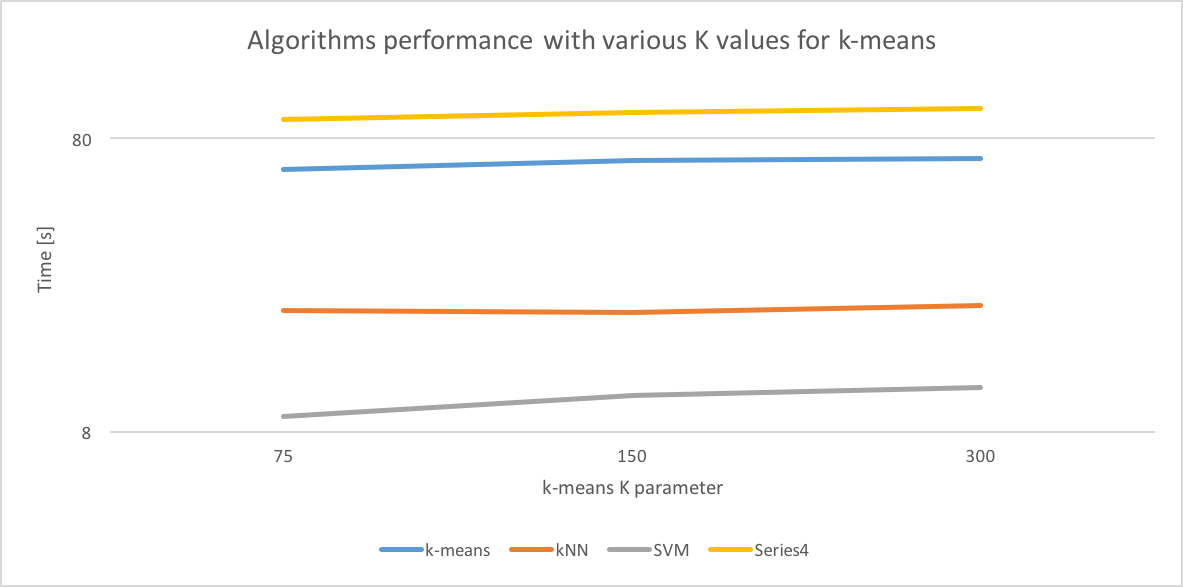
\includegraphics[width=0.9\linewidth]{images/tests/param-kmeans.png}
		\caption{Algorithms performance with various K values for k-means algorithm}
		\label{param-kmeans}
	\end{center}
\end{figure}

Test results indicate that increasing \textit{k} parameter in k-means brings small recall improvement for both kNN and SVM classificators, however the change is marginal (\ref{tests:param:kmeans}). Also, increasing \textit{k} does not affect processing time.

% \usepackage{booktabs}
% \usepackage{multirow}
\begin{table}[H]
	\centering
	\caption{kNN and SVM effectiveness with different K value in kNN}
	\label{tests:param:knn}
	\begin{tabular}{@{}lllll@{}}
		\toprule
		\multicolumn{2}{l}{K value in kNN} & 10   & 20   & 40   \\ \midrule
		\multirow{2}{*}{kNN}      & TP      & 0,74 & 0,79 & 0,82 \\
		& FN      & 0,26 & 0,21 & 0,19 \\
		\multirow{2}{*}{SVM}      & TP      & 0,67 & 0,71 & 0,79 \\
		& FN      & 0,33 & 0,29 & 0,21 \\ \bottomrule
	\end{tabular}
\end{table}

\begin{figure}[H]
	\begin{center}
		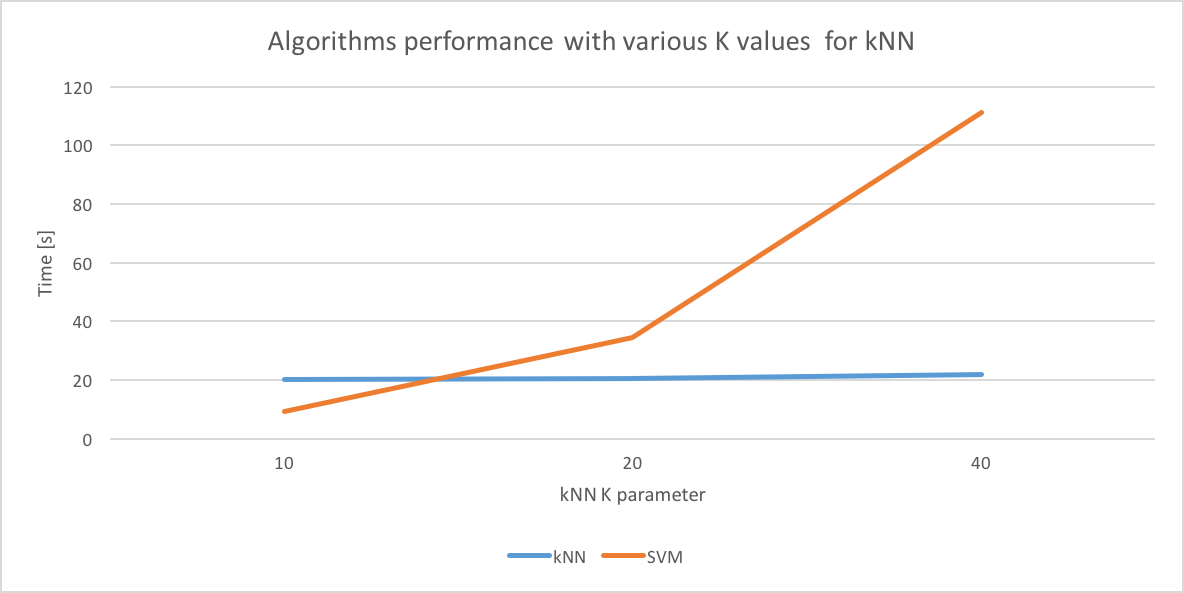
\includegraphics[width=0.9\linewidth]{images/tests/param-knn.png}
		\caption{Algorithms performance with various K values for kNN}
		\label{param-knn}
	\end{center}
\end{figure}

Changing \textit{k} parameter in kNN has more influence on results. Increasing it from 10 to 40 allows to achieve better recall for kNN by 8\% and for SVM by 12\%. Also, for kNN it does not affect total processing time, but in case of SVM it extends it significantly (21 times in presented test case).

\begin{table}[H]
	\centering
	\caption{SVM effectiveness with different kernels}
	\label{tests:param:svm}
	\begin{tabular}{@{}lllll@{}}
		\toprule
		\multicolumn{2}{l}{SVM kernel} & linear & rbf  & poly \\ \midrule
		\multirow{2}{*}{SVM}    & TP   & 0,7    & 0,71 & 0,71 \\
		& FN   & 0,3    & 0,29 & 0,29 \\ \bottomrule
	\end{tabular}
\end{table}

\begin{figure}[H]
	\begin{center}
		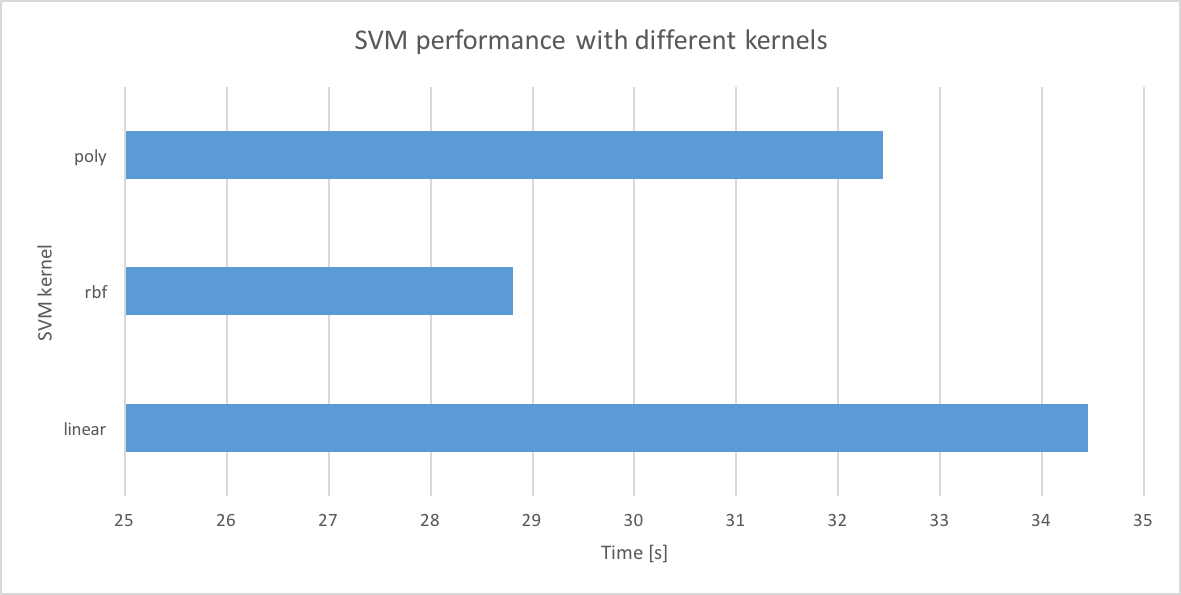
\includegraphics[width=0.9\linewidth]{images/tests/param-svm.png}
		\caption{Algorithms performance with various SVM kernels}
		\label{param-svm}
	\end{center}
\end{figure}

Last case tested whether there can be gained recall when changing kernels with which SVM works. Tests indicates, that final results were not affected by these changes, but there were significant processing time fluctuations.

\section{Conclusion}
Thic chapter outlines test cases used to verify system performance and classification algorithms accuracy with different configurations. Tests were conducted in a function of number of clusters and number of nearest neighbours and SVM kernels.
